\subsection{Arquitetura}

%
% Archtecture
%
\begin{frame}\frametitle{Arquitetura Openflow}

    \begin{itemize}
    \item Temos dois papeis principais:
        \begin{itemize}
        \item Controlador
        \item Switch Openflow
        \end{itemize}
    \item Algo te lembra plano de dados e controle desacoplados?
    \end{itemize}
    
	\begin{figure}[h]
        \centering
        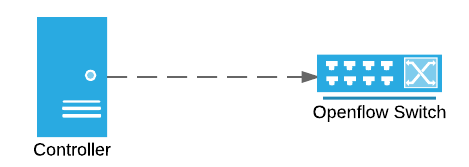
\includegraphics[scale=0.6]{images/controller-to-openflow.png}
    \end{figure}
\end{frame}



%
% Switch Archtecture
%
\begin{frame}\frametitle{Arquitetura do Switch Openflow}

    \begin{itemize}
    \item Internamente um Switch openflow é assim:
    \end{itemize}
    
	\begin{figure}[h]
        \centering
        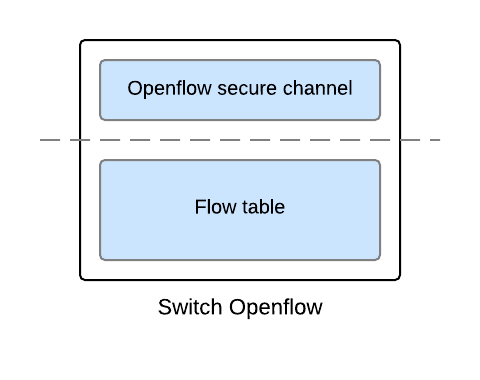
\includegraphics[scale=0.5]{images/openflow-switch-architecture.png}
    \end{figure}
\end{frame}

%
% Switch Archtecture
%
\begin{frame}\frametitle{Arquitetura Openflow}

    \begin{itemize}
    \item \textbf{Openflow secure channel}: É a conexão segura entre o
          controlador e o switch openflow
    \vspace*{0.5cm}
    \item \textbf{Flow table}: É a tabela onde são identificados os fluxos
    \vspace*{0.5cm}
    \item Para cada fluxo tem-se uma ação (action) a ser tomada
    \end{itemize}
\end{frame}

%
% Switch Archtecture
%
\begin{frame}\frametitle{Arquitetura Openflow}

    \begin{itemize}
    \item Um fluxo é identificado pelos seguintes campos do cabeçalho 
          Openflow:
    \end{itemize}
	\begin{figure}[h]\hspace*{-1.2cm}
        \centering
        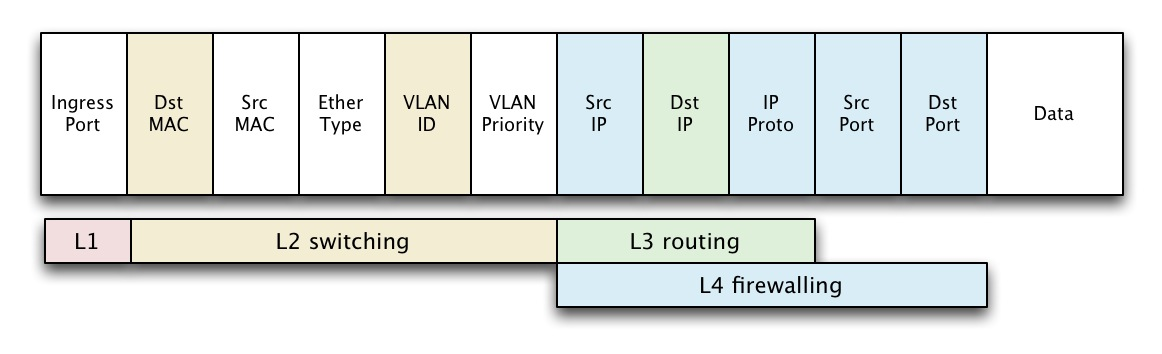
\includegraphics[scale=0.32]{images/openflow-header.jpg}
    \end{figure}
    
\end{frame}


%
% Actions
%
\begin{frame}\frametitle{Actions}

	\begin{figure}[h]
        \centering
        
\includegraphics[scale=0.5]{images/action.png}
    \end{figure}
    
\end{frame}


%
% Actions
%
\begin{frame}\frametitle{Tipos de Actions}

    \begin{itemize}
    \item Forwarding
    \item Drop
    \item Set
    \item strip
    \item Copy-in
    \item Copy-out
    \item Push
    \item Pop
    \item Dec
    \end{itemize}

\end{frame}


%
% Flow table 
%
\begin{frame}\frametitle{Tabela de Fluxos}

\begin{center}
    \begin{tabular}{ | l | l | l | l |}
    \hline
    \textbf{Header} & \textbf{Counters} & \textbf{Actions} & \textbf{Priority} \\ \hline
    in\_port=5 & 55635 bytes & \pbox{20cm}{Forward \\ port=8} & 100 \\ \hline
    \pbox{20cm}{ip=192.168.1.42 \\ port=80} & 4032 bytes & \pbox{30cm}{Set \\ rewrite \\ ip=192.168.1.100} & 500 \\ \hline
    ipproto=UDP & 100 bytes & Drop & 700 \\ \hline
    \end{tabular}
\end{center}

\end{frame}

%
% Controller
%
\begin{frame}\frametitle{Controlador}

    \begin{itemize}
    \item É um software que se conecta de maneira segura ao switch openflow
          com o objetivo de manipular sua tabela de fluxos
    \item Esse software pode ser distribuído
    \item Ele representa uma entidade lógica e centralizada
    \item É possível ter visão e controle de estado global da rede
    \item Permite que outros serviços e programas façam requisições e troca
          de mensagem com o plano de controle da rede
    \item Pode calcular estatísticas da rede
    
    \end{itemize}

\end{frame}


%
% Controller
%
\begin{frame}\frametitle{Controlador}

    \begin{itemize}
    \item Cabe ao programador lidar com os problemas típicos em 
          desenvolvimento de software:
          \begin{itemize}
          \item Tolerância a falha
          \item Persistência
          \item Eficiência
          \item design de implementação
          \item debugging
          \item Testes
          \end{itemize}
    \end{itemize}
\end{frame}

%
% Controller
%
\begin{frame}\frametitle{Controlador}

    \begin{itemize}
    \item Controladores Openflow:
          \begin{itemize}
          \item Biblioteca \href{http://opennetworkingfoundation.github.io/libfluid/index.html}{Libfluid}
                para criação de aplicações/controladores em SDN
          \item \href{http://www.noxrepo.org/nox/about-nox/}{Nox Controller}
          \item \href{https://openflow.stanford.edu/display/Beacon/Home}{Beacon}
          \item \href{http://www.noxrepo.org/pox/about-pox/}{Pox Controller}
          \item \href{http://osrg.github.io/ryu/}{Ryu}
          \end{itemize}
    \end{itemize}
\end{frame}


%
% Simple topology
%
\begin{frame}\frametitle{Arquitetura Openflow}

    \begin{itemize}
    \item Uma topologia simples:
    \end{itemize}
    
	\begin{figure}[h]
        \centering
        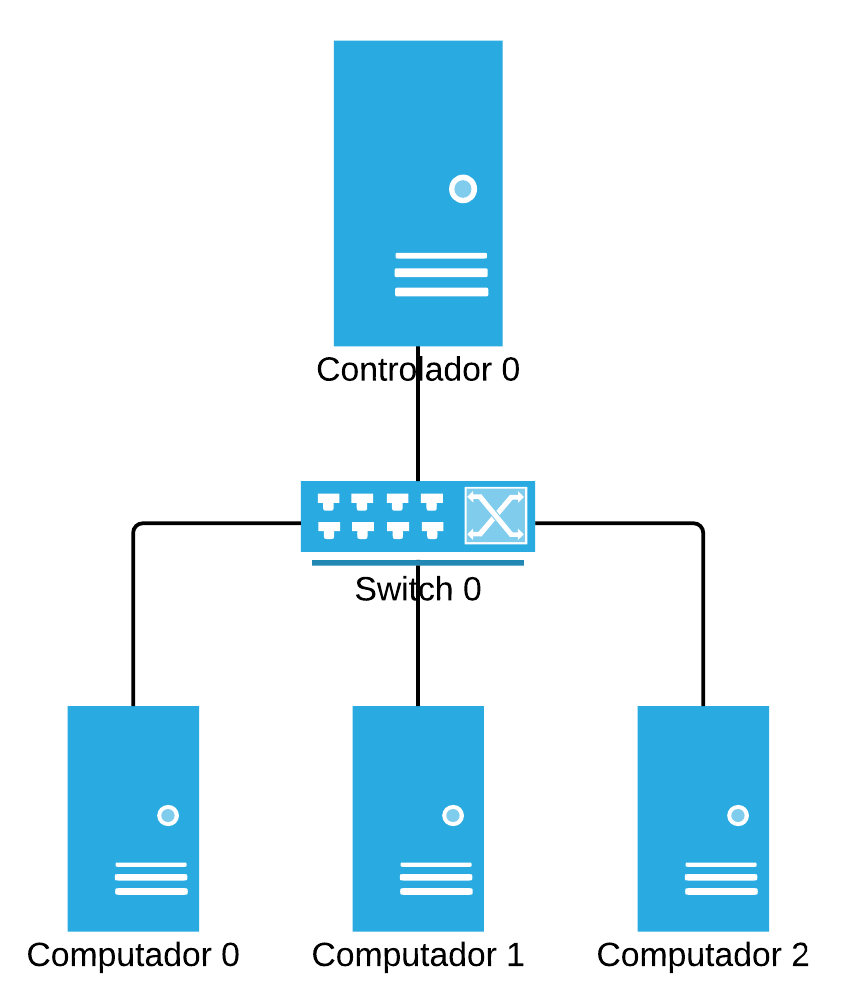
\includegraphics[scale=0.3]{images/simple-topology.png}
    \end{figure}
\end{frame}


%
% N openflow 
%
\begin{frame}\frametitle{Arquitetura Openflow}

    \begin{itemize}
    \item Um controlador para vários \emph{Switches}
    \end{itemize}
    
	\begin{figure}[h]
        \centering
        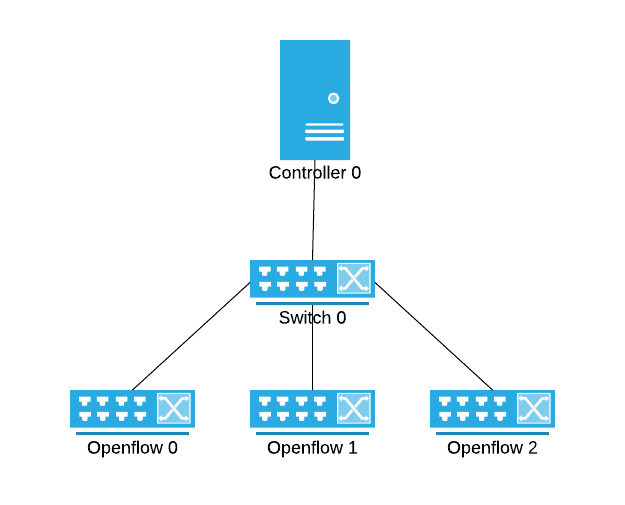
\includegraphics[scale=0.4]{images/n-openflow-switches.png}
    \end{figure}
\end{frame}


%
% SDN inter domain
%
\begin{frame}\frametitle{Arquitetura Openflow}

    \begin{itemize}
    \item Comunicação entre domínios de rede
    \end{itemize}
    
   
	\begin{figure}[h]\hspace*{-1cm}
        \centering
        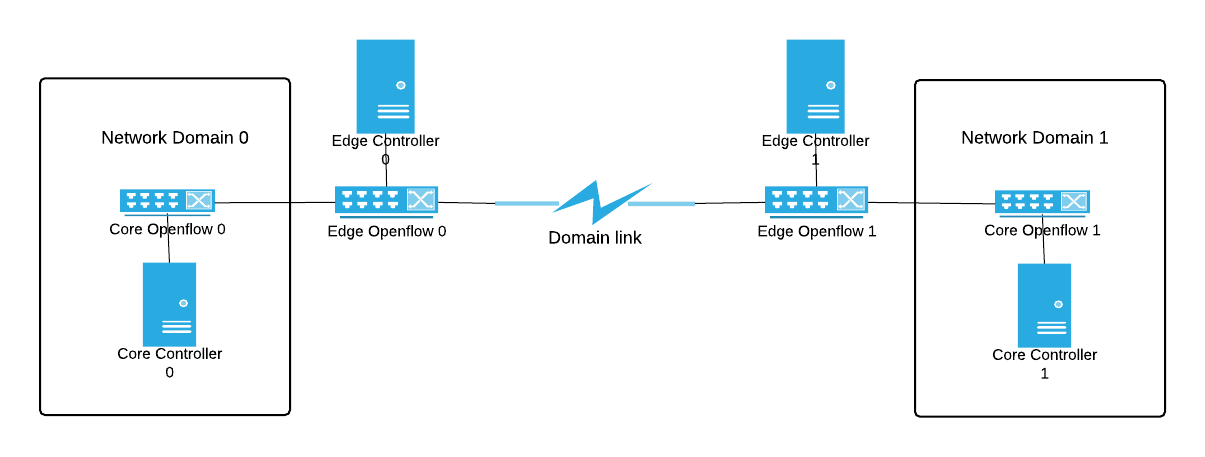
\includegraphics[scale=0.3]{images/edge-core-sdn.png}
    \end{figure}
\end{frame}



%
% Distributed openflow controller
%
\begin{frame}\frametitle{Arquitetura Openflow}

    \begin{itemize}
    \item Controlador distribuído
    \end{itemize}
    
	\begin{figure}[h]
        \centering
        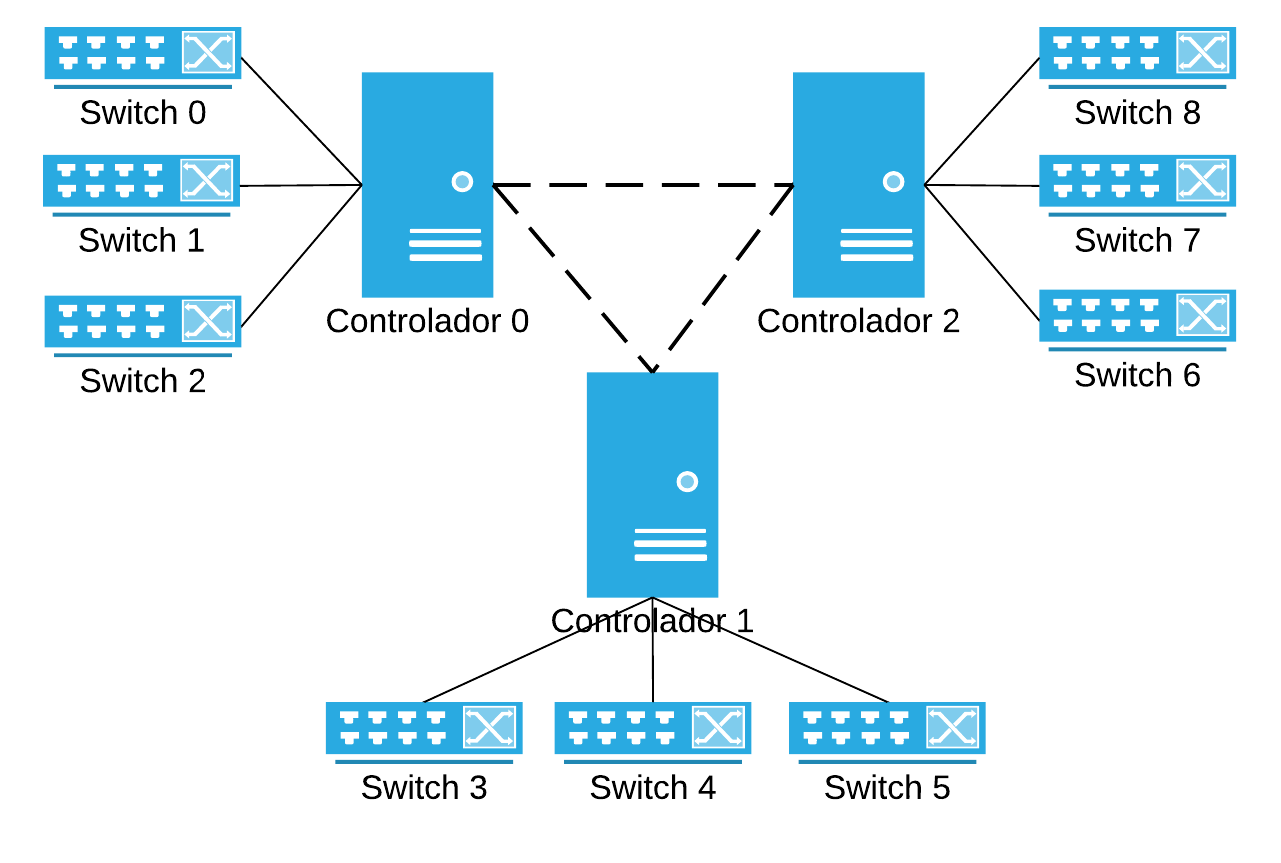
\includegraphics[scale=0.4]{images/distributed_sdn_controller.png}
    \end{figure}
\end{frame}
